% This presentation uses Aalborg Beamer Theme http://kom.aau.dk/~jkn/latex/latex.php#beamer_aausidebar
\documentclass[]{beamer}
\usetheme[
%%% options passed to the outer theme
hidetitle,           % hide the (short) title in the sidebar
hideauthor,          % hide the (short) author in the sidebar
%    hideinstitute,       % hide the (short) institute in the bottom of the sidebar
%    shownavsym,          % show the navigation symbols
%    width=2cm,           % width of the sidebar (default is 2 cm)
%    hideothersubsections, % hide all subsections but the subsections in the current section
hideallsubsections,  % hide all subsections
%    left                % right of left position of sidebar (default is right)
  ]{Aalborg}
  
% If you want to change the colors of the various elements in the theme, edit and uncomment the following lines
% Change the bar and sidebar colors:
\definecolor{MyBlue}{RGB}{0,53,107}
\definecolor{MyLightBlue}{RGB}{0,53,107}
\definecolor{MyGray}{RGB}{102,102,102}
\setbeamercolor{Aalborg}{fg=MyLightBlue!50, bg=MyBlue}
%\setbeamercolor{sidebar}{bg=red!20}
% Change the color of the structural elements:
\setbeamercolor{structure}{fg=MyBlue}
% Change the frame title text color:
\setbeamercolor{frametitle}{fg=MyBlue}
\setbeamercolor{titlepagecolorbox}{fg=white,bg=MyBlue}
% Change the normal text color background:
%\setbeamercolor{normal text}{fg=gray!50}
% ... and you can of course change a lot more - see the beamer user manual.

\usepackage[utf8]{inputenc}
\usepackage[english, ukrainian]{babel}
\usepackage[T1, T2A]{fontenc}
% Or whatever. Note that the encoding and the font should match. If T1
% does not look nice, try deleting the line with the fontenc.
\usepackage{xcolor}
\usepackage[]{graphicx}
\usepackage{booktabs}
\usepackage{scalerel}
\usepackage[normalem]{ulem}
\usepackage{mathtools}
\def\thumbsup{\scalerel*{\includegraphics{pres_figures/up.png}}{O}}
\def\thumbsdown{\scalerel*{\includegraphics{pres_figures/down.png}}{g}}

\usepackage{droid}
\usepackage[backend=bibtex,style=authoryear-icomp, sorting=nyt]{biblatex}
\setbeamertemplate{caption}{\insertcaption} 
\addbibresource{pres-references.bib}

% colored hyperlinks
\newcommand{\chref}[2]{%
  \href{#1}{{\usebeamercolor[bg]{Aalborg}#2}}%
}

% footnotes without markers
\newcommand\blfootnote[1]{%
	\begingroup
	\renewcommand\thefootnote{}\footnote{#1}%
	\addtocounter{footnote}{-1}%
	\endgroup
}

\title{\textbf{Підхід до швидкого одновимірного аналізу просторової конфігурації\\
		       ландшафтних градієнтів}}

\date[25 жовтня 2017 р.]{\vspace{-1.5 mm} 26 жовтня 2017~р.\\
	                    {\href{http://gc.igs-nas.org.ua/}
	                    {\vspace{-1.5 mm}\scriptsize Ідеї та новації в системі наук про Землю}\\
                        {\scriptsize м.~Київ, Україна}}}
                                        
\author[Дар'я Свідзінська] % optional, use only with lots of authors
{
  Дар'я Свідзінська\\
  \href{mailto:d.svidzinska@gmail.com}{{\tt d.svidzinska@gmail.com}}
}

\institute[
%  {\includegraphics[scale=0.2]{aau_segl}}\\ %insert a company, department or university logo
  % Кафедра фізичної географії та геоекології\\
  % Лабораторія GeoForAll\\
  % Київський національний університет імені Тараса Шевченка
] % optional - is placed in the bottom of the sidebar on every slide
{% is placed on the bottom of the title page
  Кафедра фізичної географії та геоекології\\
  \href{http://lab.osgeo.org.ua/}{Лабораторія GeoForAll}\\
  Київський національний університет імені Тараса Шевченка
  
  %there must be an empty line above this line - otherwise some unwanted space is added between the university and the country (I do not know why;( )
}


% specify the logo in the top right/left of the slide
%\pgfdeclareimage[height=1cm]{mainlogo}{AAUgraphics/aau_logo_new} % placed in the upper left/right corner
%\logo{\pgfuseimage{mainlogo}}

% specify a logo on the titlepage (you can specify additional logos an include them in 
% institute command below
% \pgfdeclareimage[height=1.5cm]{titlepagelogo}{AAUgraphics/tsnuk_logo} % placed on the title page
% \pgfdeclareimage[height=1.5cm]{titlepagelogo2}{AAUgraphics/lab_logo} % placed on the title page
% \titlegraphic{% is placed on the bottom of the title page
	%\pgfuseimage{titlepagelogo}
	%\hspace{0.5cm}\pgfuseimage{titlepagelogo2}
%}

\begin{document}
    
	% the titlepage
	{%\aauwavesbg
		\begin{frame}[plain,noframenumbering] % the plain option removes the sidebar and header from the title page
		\titlepage
\end{frame}}
%%%%%%%%%%%%%%%%

\section{Вихідні положення}
\subsection{Ландшафтний градієнт}
\begin{frame}{Ландшафтний градієнт}{Поняття та аналітичний потенціал}

\textbf{Ландшафтний градієнт} -- континуальна поверхня, що кількісно описує зміну певної характеристики ландшафту в просторі географічних координат.\footcites{Cushman2010}{Lausch2015}{Muller1998}

\begin{columns}[c]
	
	\column{.5\textwidth}
	
	\thumbsup \hspace{0.2 cm} \textbf{Переваги:}
	
	\begin{itemize}
		\item \sout{однорідні ділянки}
		\item \sout{чіткі межі}
		\item дані ДЗЗ
		\item геостатистика
		\item багатовимірний аналіз
		\item екологічний аналіз		
	\end{itemize}
	
	\column{.5\textwidth}
	
	\thumbsdown \hspace{0.2 cm} \textbf{Недоліки:}
	
	\begin{itemize}
		\item поглиблений аналітичний досвід
		\item складні набори даних
		\item великі об'єми даних
		\item нестандартизовані показники
		\item складна інтерпретація
	\end{itemize}
	
\end{columns}


\end{frame}
%%%%%%%%%%%%%%%%

\subsection{Semivariance}
\begin{frame}{Функції структури одновимірних даних}{Semivariance}

\textbf{Semivariance}\footnote{можливі варанти перекладу -- семіваріація, напівваріація, напівдисперсія} -- середня дисперсія, розрахована за всіма парами точок, розділеними заданою відстанню (лагом)\footcite{Legendre2012}

%$$ \gamma(h) = \frac{\sum\limits_{i = 1}^{N(h)}(z_i - z_{i+h})^2}{2N(h)} $$

\begin{itemize}
	\item міра дисперсії просторової змінної 
	\item розраховується як функція відстані
	\item візуалізується як варіограма 
	\item варіабельність значень, як функція масштабу
	\item допомагає встановити гіпотетичний \textcolor{MyBlue}{зв'язок між просторовою структурою та процесом}, що її генерує
\end{itemize}

\end{frame}
%%%%%%%%%%%%%%%%

\subsection{Автокореляція}
\begin{frame}{Функції структури одновимірних даних}{Автокореляція}

\textbf{Автокореляція} -- кореляція, розрахована за всіма парами точок, розділеними заданою відстанню (лагом)\footcite{Legendre2012}

%$$ r(h) = corr[z_i, z_{i+h}] $$

\begin{itemize}
	\item міра \textit{авто}кореляції просторової змінної 
	\item розраховується як функція відстані
	\item візуалізується як корелограма 
	\item залежність значень, як функція масштабу
	\item спростовує \textcolor{MyBlue}{наявність або відсутність просторової структури}
	\item ідентифікує \textcolor{MyBlue}{критичні відстані} на яких спостерігається значуща позитивна або негативна кореляція
\end{itemize}

\end{frame}
%%%%%%%%%%%%%%%%

\section{Мета та завдання}
\begin{frame}{Мета та завдання роботи}{}
\textcolor{MyBlue}{Мета} -- розробити, алгоритмізувати та апробувати підхід, який полегшить розв'язання наступних аналітичних питань:
	\begin{enumerate}
		\item Як визначити оптимальний об'єм вибірки для аналізу?
		\item Якщо об'єм вибірки занадто великий, чи можливо його зменшити і як?
		\item Як визначити оптимальний лаг та кількість класів відстані?
		\item За якими параметрами оцінювати надійність та значущість отриманих значень?
		\item Як полегшити інтерпретацію результатів?		
    \end{enumerate}
\end{frame}
%%%%%%%%%%%%%%%%

\section{Територія}
\begin{frame}{Канівський природний заповідник}{Нагірна природоохоронна дільниця та її околиці}
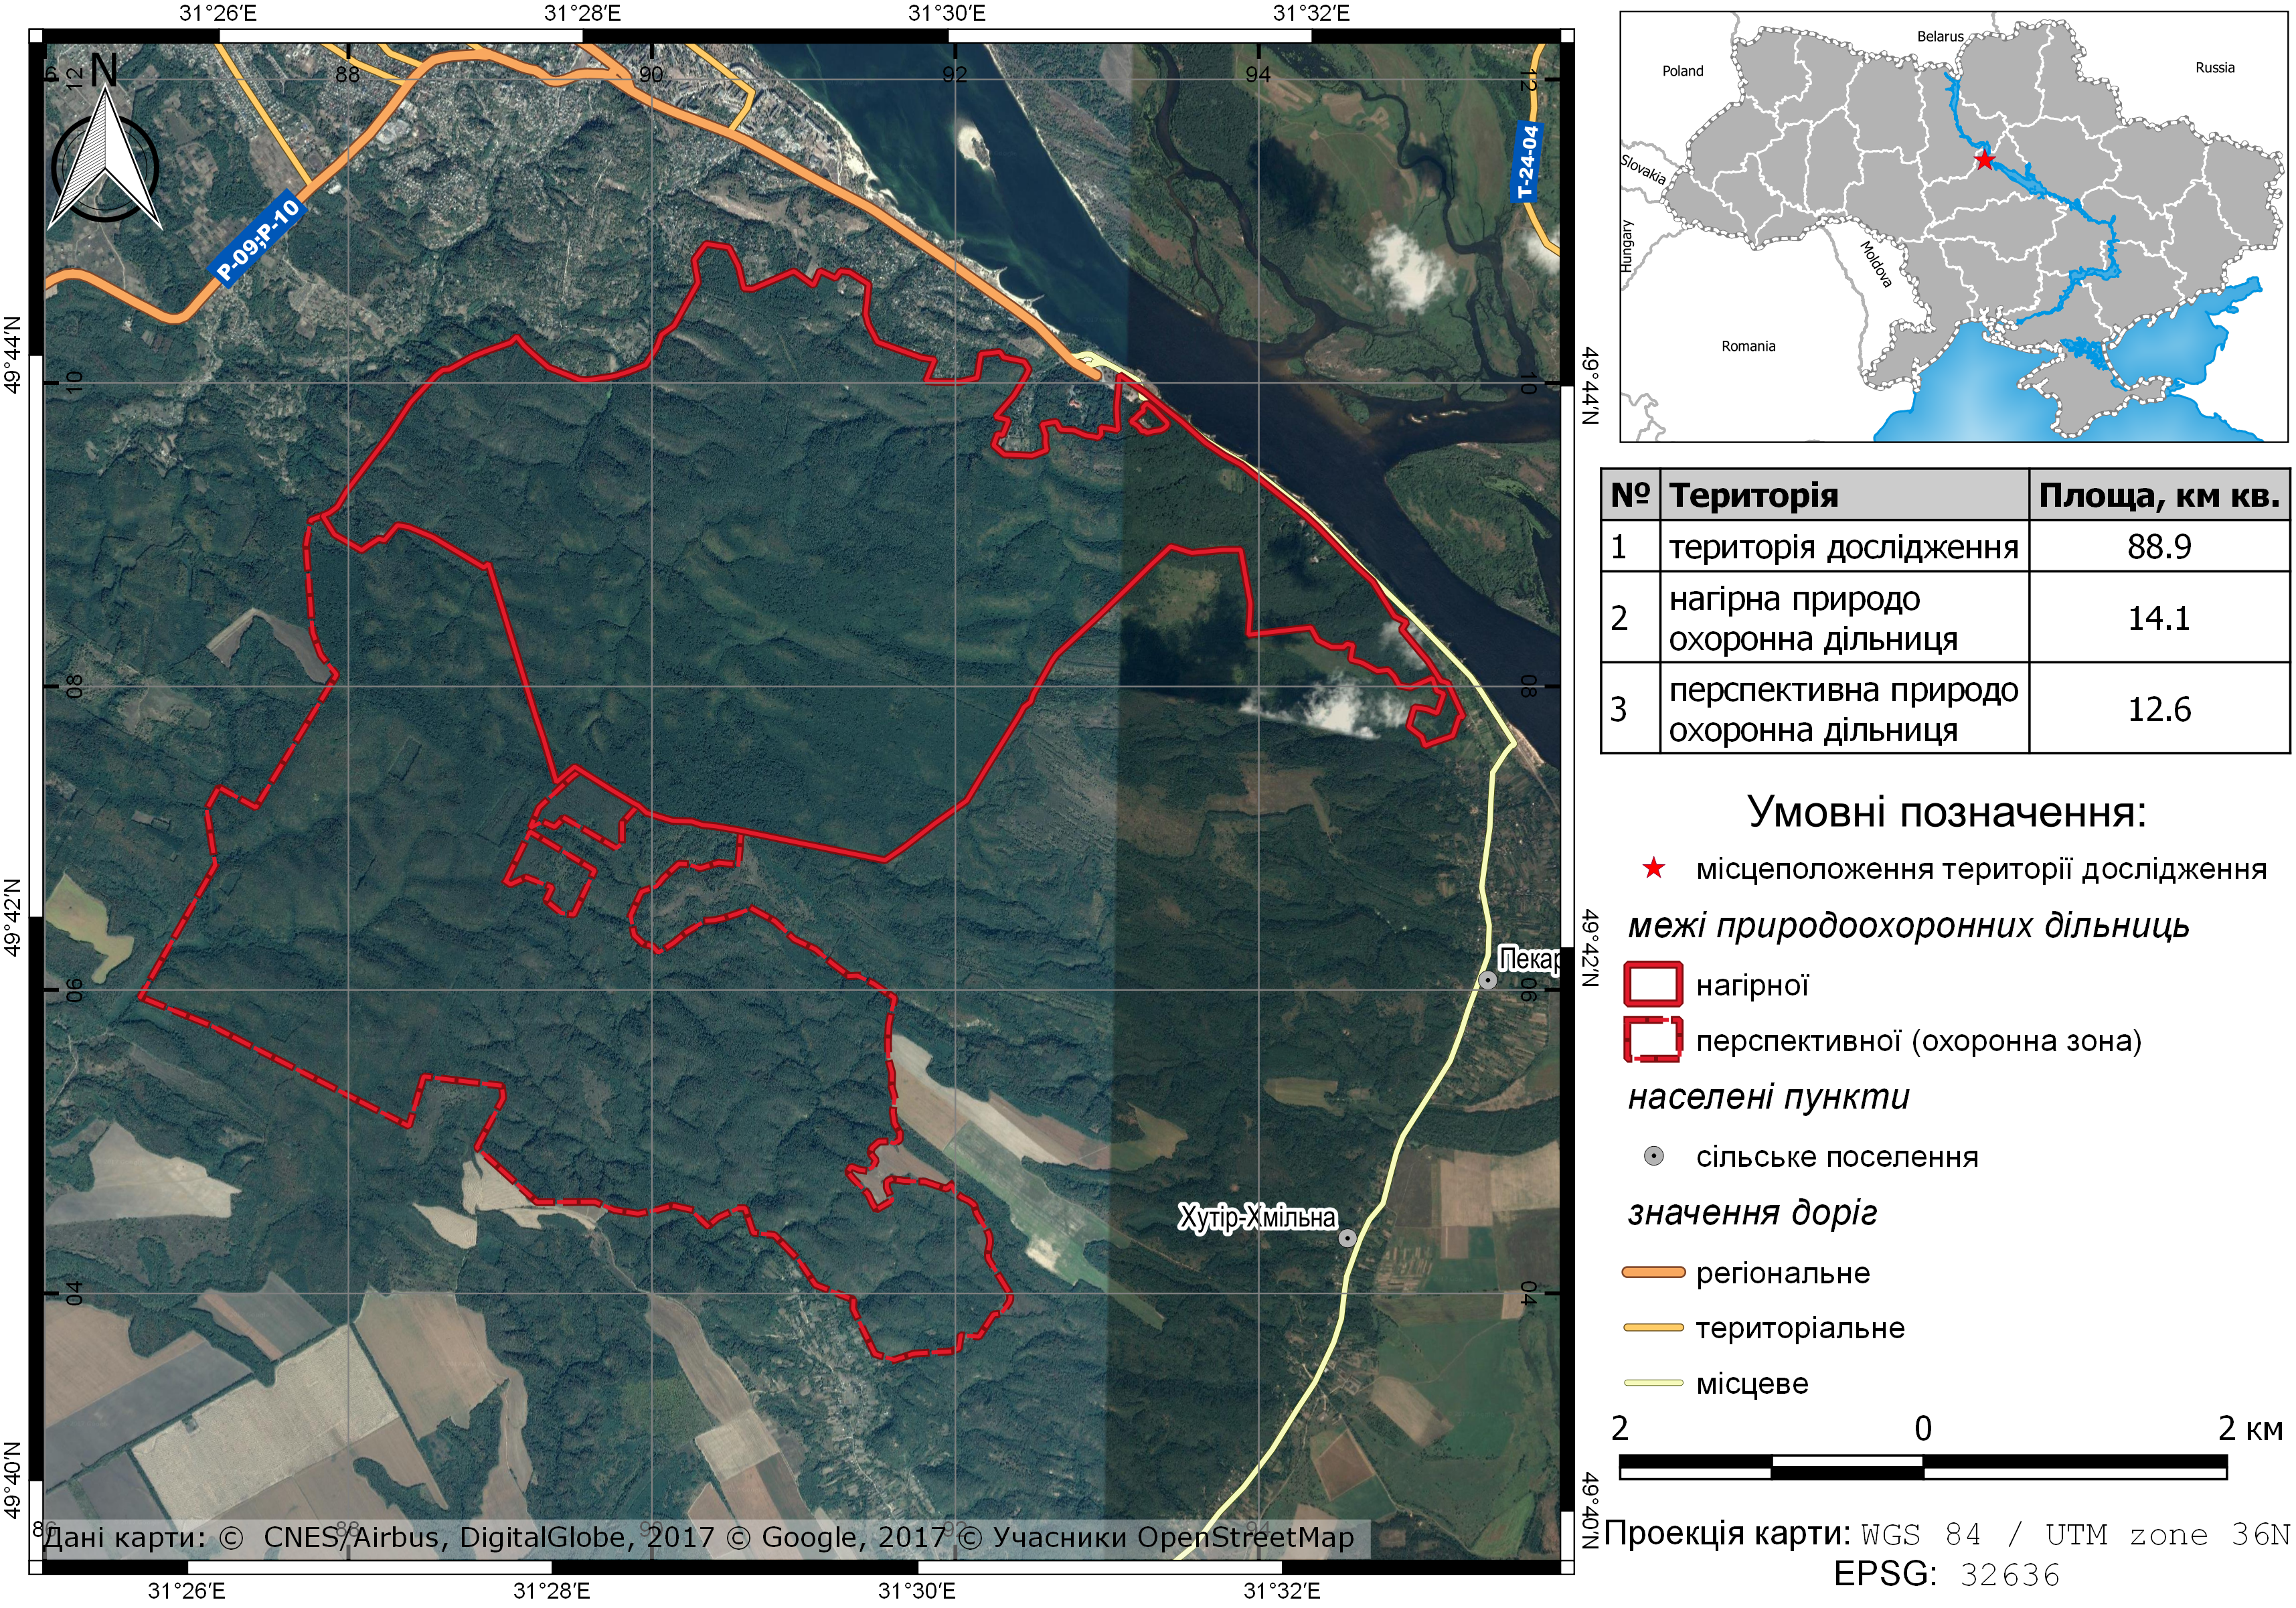
\includegraphics[width=\textwidth]{./pres_figures/area_map.png}
\end{frame}
%%%%%%%%%%%%%%%%

\section{Матеріали}
\begin{frame}{Матеріали дослідження}{Похідні ЦМВ AW3D30 та EVI}
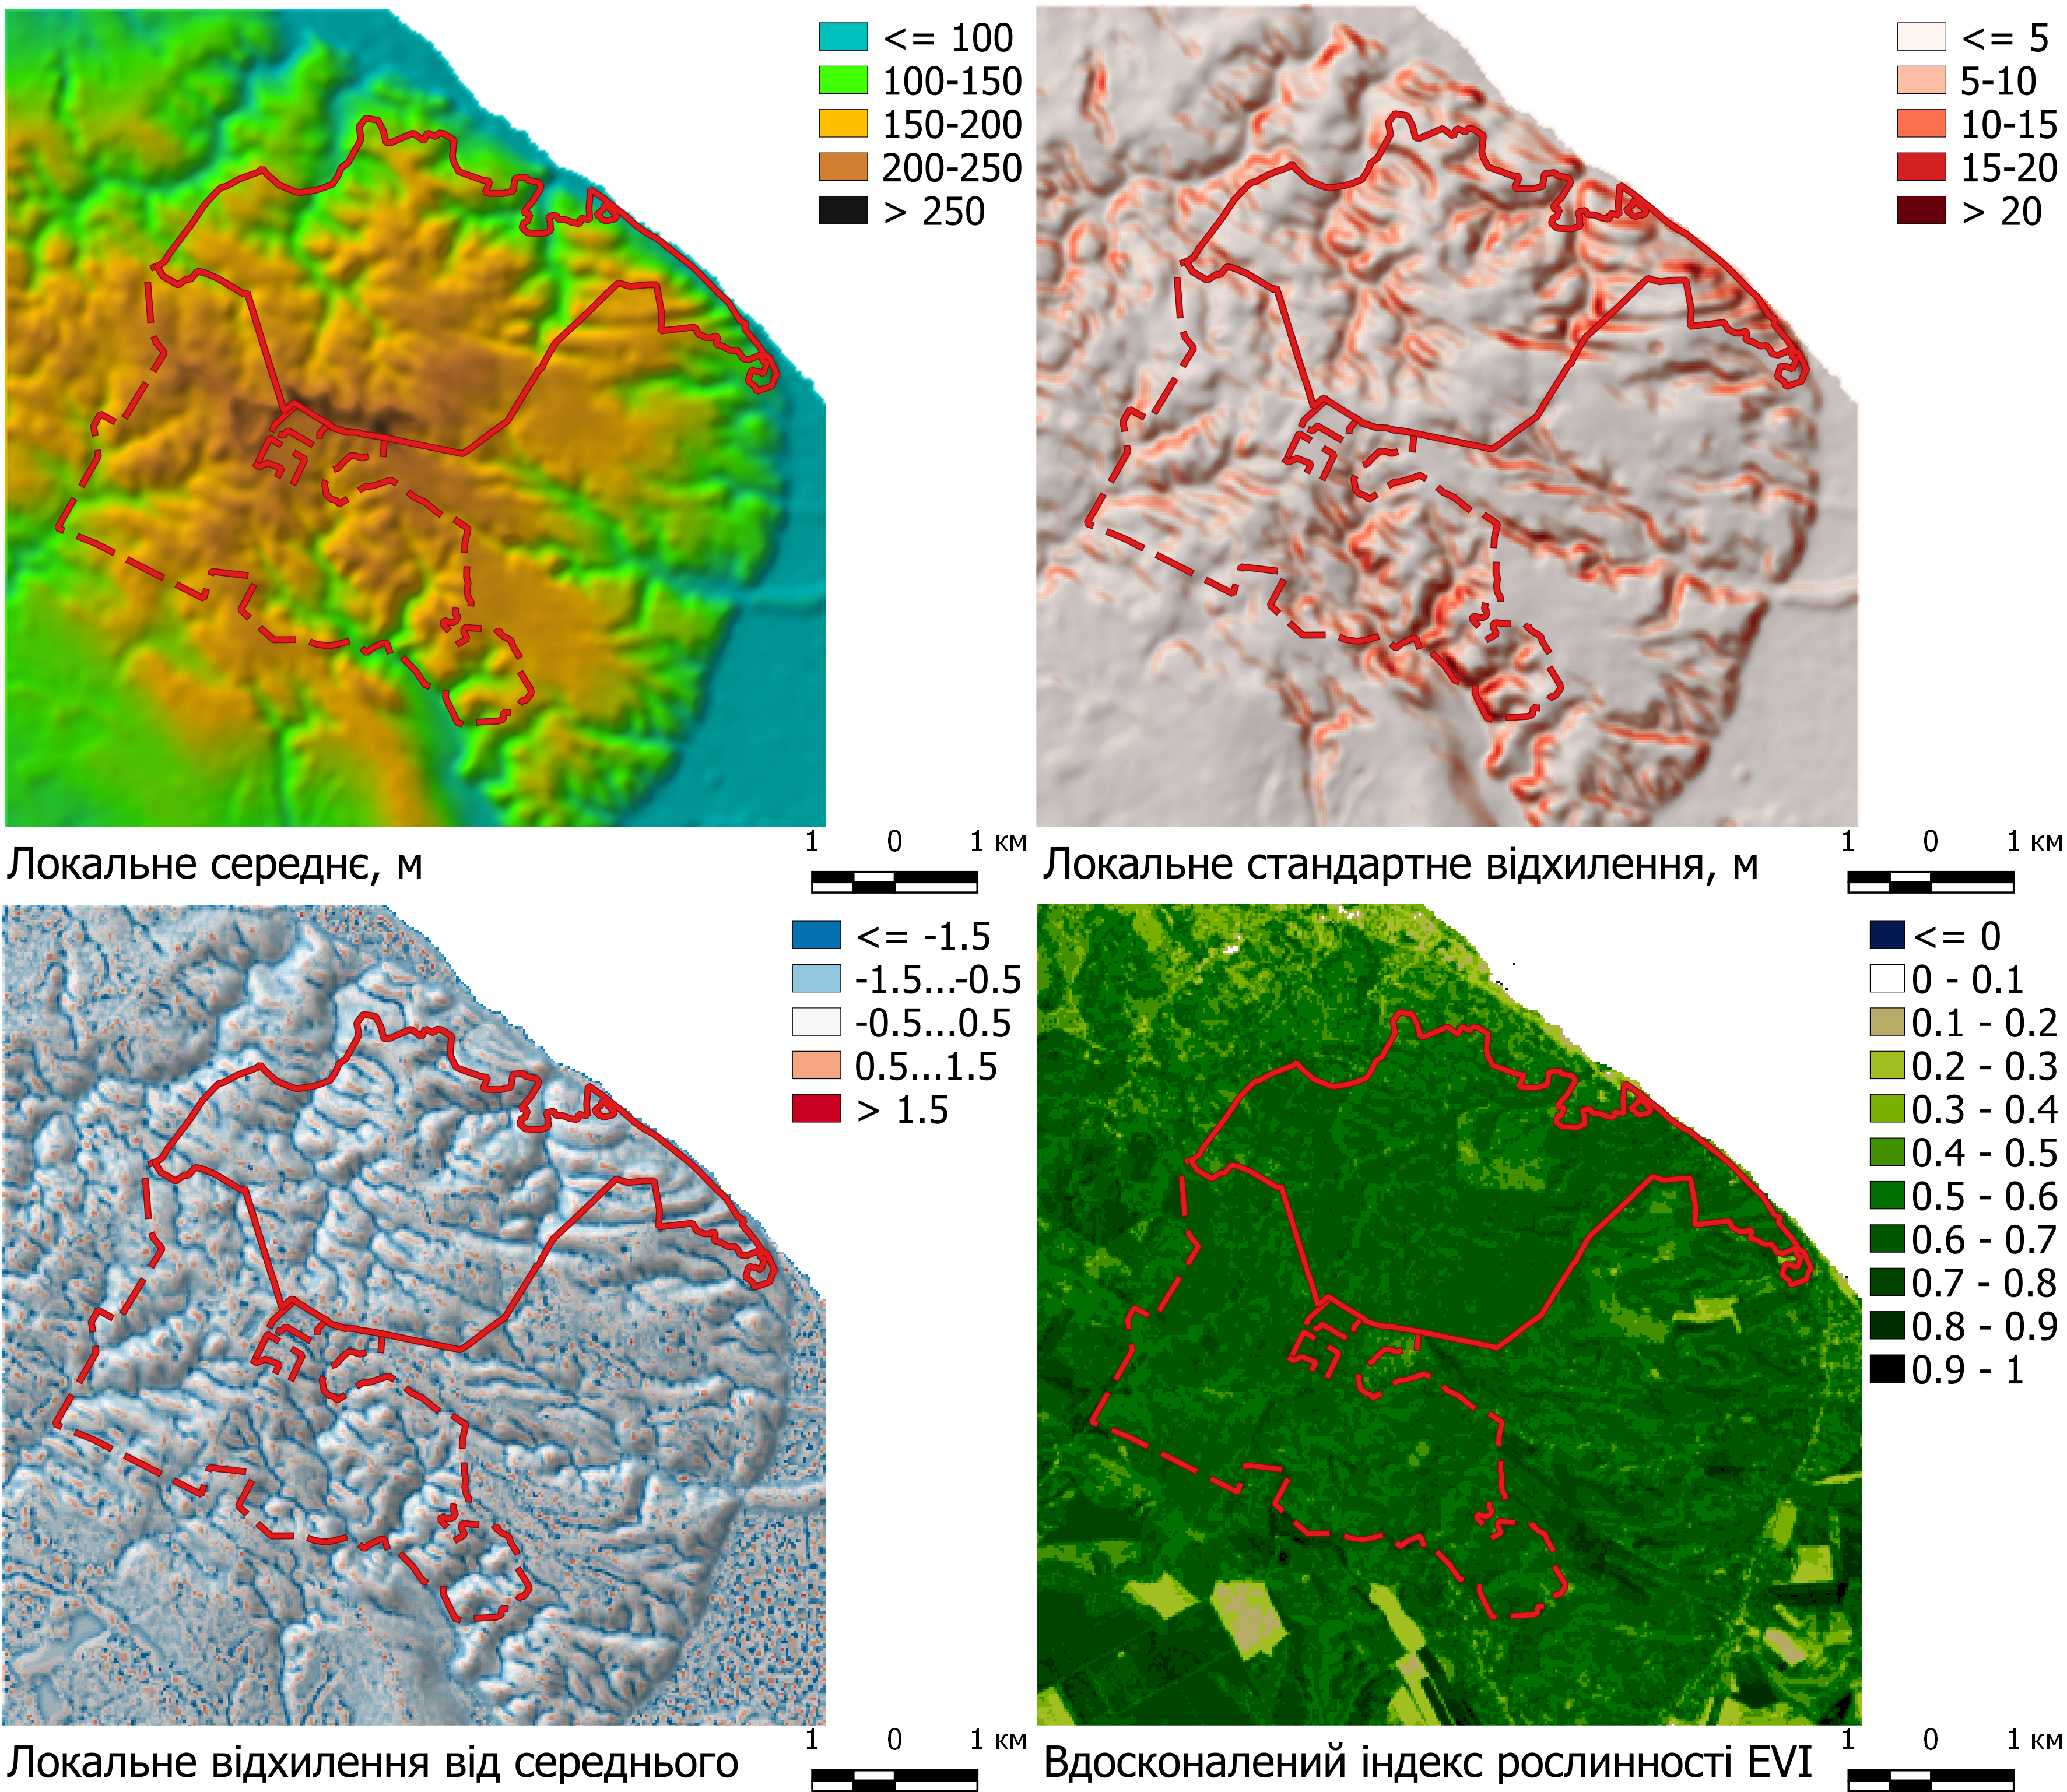
\includegraphics[width=0.85\textwidth]{./pres_figures/gradients_map.png}
\blfootnote{\tiny{\cites{Conrad2015}{EorcJaxa2017}{Lecours2017}{Vermote2016}}}
\end{frame}
%%%%%%%%%%%%%%%%

\section{Методи}
\subsection{Програмне середовище мови R}
\begin{frame}{Методи дослідження}{Програмне середовище мови R}
\includegraphics[width=1.0cm]{./pres_figures/R_logo.png} -- програмне середовище для статистичних обчислень та графіки\footcites{Rcite2017}{EcoGenetics2017}{geoR2016}{Wickham2009}{inlmisc2017}{raster2016}{rgdal2017}{Pebesma2005}{Bivand2013}:
\begin{itemize}
	\item \texttt{EcoGenetics} -- корелограми
	\item \texttt{geoR} -- варіограми
	\item \texttt{ggplot2} -- аналітична візуаліація
	\item \texttt{inlmsc} -- вибірки за профілями
	\item \texttt{raster} -- робота з растрами, формування вибірок
	\item \texttt{rgdal} -- експорт результатів у ESRI shape
	\item \texttt{sp} -- побудова ліній профілів
\end{itemize}
\end{frame}
%%%%%%%%%%%%%%%%

\subsection{Алгоритм аналізу}
\begin{frame}{Методи дослідження}{Алгоритм аналізу}
\includegraphics[width=\textwidth]{./pres_figures/algorithm_flowchart.png}
\blfootnote{\href{https://github.com/darsvid/univariate_structure_functions}{ https://github.com/darsvid/univariate\_structure\_functions}}
\end{frame}
%%%%%%%%%%%%%%%%

\section{Результати}
\subsection{Параметри розрахунку}
\begin{frame}{Результати дослідження}{Параметри розрахунку}

\begin{table}
	\caption{Параметри розрахунку semivariance}
	\vspace{-0.5cm}
	\resizebox{\linewidth}{!}{
	\begin{tabular}{l | l l l l l l l}
		Градієнт & $\alpha$ & $N_1$ & $R$ & $N_2$ & $h$ & $n$ & $L$ \\
		\hline \hline
		середнє & 0.01 & $3\,959$ & -- & -- & 310 & 23 & $7\,130$ \\ \hline
		стандартне відхилення & 0.01 & $20\,412$ & 112.9 & $1\,858$ & 340 & 21 & $7\,140$ \\ \hline
		відхилення від середнього & -- & -- & -- & $3\,000$ & 310 & 23 & $7\,130$ \\ \hline
		evi & 0.01 & $2\,163$ & -- & -- & 320 & 22 & $7\,140$ \\ \hline
    \end{tabular}}
\end{table}
\vspace{-0.5cm}
\begin{table}
	\caption{Параметри розрахунку автокореляції}
	\vspace{-0.5cm}
	\resizebox{\linewidth}{!}{
		\begin{tabular}{l | l l l l l l l}
			Градієнт & $\alpha$ & $N_1$ & $R$ & $N_2$ & $h$ & $n$ & $L$ \\
			\hline \hline
			середнє & 0.001 & $83\,397$ & 112.9 & 808 & 370 & 19 & $7\,030$ \\ \hline
			стандартне відхилення & 0.01 & $20\,412$ & 112.9 & $1\,858$ & 340 & 21 & $7\,140$ \\ \hline
			відхилення від середнього & -- & -- & -- & $3\,000$ & 310 & 23 & $7\,130$ \\ \hline
			evi & 0.01 & $2\,163$ & -- & -- & 320 & 22 & $7\,140$ \\ \hline
	\end{tabular}}
\end{table}

\small{де $\alpha$ -- рівень значущості; $N_1$ та $N_2$ -- розмір вибірки без та з урахуванням автокореляції в радіусі $R$; $h$ -- лаг; $n$ -- кількість класів відстані; $L$ -- максимальна відстань}

%\blfootnote{\href{https://github.com/darsvid/univariate_structure_functions}{https://github.com/darsvid/univariate\_structure\_functions}}
\end{frame}
%%%%%%%%%%%%%%%%
\subsection{Просторова конфігурація}
\subsubsection{Локальне середнє}
%%%%%%%%%%%%%%%%
\begin{frame}{Локальне середнє}{Профілі}
	\includegraphics[width=\textwidth]{./pres_figures/plots_mean/profiles_plot.png}%
\end{frame}
%%%%%%%%%%%%%%%%

\begin{frame}{Локальне середнє}{Просторова конфігурація}
    \includegraphics[width=\textwidth]{./pres_figures/plots_mean/mean_all.png}%
    
    \begin{itemize}
    	\item масштаб просторової залежності 4~000--5~000~м
    	\item відсутність автокореляції 3~500--3~800~м
    	\item істотна додатна кореляція до 500~м
    \end{itemize}
\end{frame}
%%%%%%%%%%%%%%%%

\subsubsection{Локальне стандартне відхилення}
%%%%%%%%%%%%%%%%
\begin{frame}{Локальне стандартне відхилення}{Профілі}
\includegraphics[width=0.92\textwidth]{./pres_figures/plots_std_dev/profiles_plot.png}%
\end{frame}
%%%%%%%%%%%%%%%%

\begin{frame}{Локальне стандартне відхилення}{Просторова конфігурація}
\includegraphics[width=\textwidth]{./pres_figures/plots_std_dev/std_dev_all.png}%

\begin{itemize}
\item масштаб просторової залежності 1~000~м
\item відсутність автокореляції 1~750--2~250~м
\item середня додатна кореляція до 250~м
%\item лінійний градієнт до 1~500--2~000~м, а далі -- випадкові значення
\end{itemize}
\end{frame}
%%%%%%%%%%%%%%%%

\subsubsection{Локальне відхилення від середнього}
%%%%%%%%%%%%%%%%
\begin{frame}{Локальне відхилення від середнього}{Профілі}
\includegraphics[width=0.91\textwidth]{./pres_figures/plots_dev_from_mean/profiles_plot.png}%
\end{frame}
%%%%%%%%%%%%%%%%

\begin{frame}{Локальне відхилення від середнього}{Просторова конфігурація}
\includegraphics[width=\textwidth]{./pres_figures/plots_dev_from_mean/dev_from_mean_all.png}%

\begin{itemize}
\item \sout{відсутня виражена просторова залежність}
\item \sout{мінімальна автокореляція}
\item \sout{провідну роль відіграє шумова компонента}
\item вибірка є недостатньою для виявлення просторової кореляції, яка може існувати  
\end{itemize}
\end{frame}
%%%%%%%%%%%%%%%%

\subsubsection{Вдосконалений індекс рослинності EVI}
%%%%%%%%%%%%%%%%
\begin{frame}{Вдосконалений індекс рослинності EVI}{Профілі}
\includegraphics[width=0.83\textwidth]{./pres_figures/plots_evi/profiles_plot.png}%
\end{frame}
%%%%%%%%%%%%%%%%

\begin{frame}{Вдосконалений індекс рослинності EVI}{Просторова конфігурація}
\includegraphics[width=\textwidth]{./pres_figures/plots_evi/evi_all.png}%

\begin{itemize}
\item масштаб просторової залежності 500--1~000~м
\item відсутність автокореляції $\sim$3~000~м
\item середня додатна автокореляція до 200~м
\item великі структурні елементи поєднані з дрібномасштабним шумом
\end{itemize}
\end{frame}
%%%%%%%%%%%%%%%%






\section{Висновки}

\begin{frame}{Висновки}{}
\begin{columns}[c]
	\column{0.6\textwidth}
	\includegraphics[width=\textwidth]{./pres_figures/grids_map.png}
	
	\column{0.4\textwidth}
	\begin{itemize}
		\item максимум автокореляції в радіусі 300~м
		\item узагальнений масштаб просторової залежності 1~000~м
		\item узагальнена нульова автокореляція 2~000~м
	\end{itemize}
\end{columns}
\end{frame}
%%%%%%%%%%%%%%%%

\section{Обговорення}
\begin{frame}{Обговорення}{}
\begin{enumerate}
	\item виявлені закономірності відповідають середньому масштабу
	\item для характеристики локальних варіацій
	\begin{itemize}
		\item більш якісні дані
		\item вища розрізненна здатність
		\item менша відстань інтересу
	\end{itemize}
	\item зберігається потреба у більш ефективних алгоритмах	
\end{enumerate}	
\end{frame}
%%%%%%%%%%%%%%%%

%\section{Посилання}
%\begin{frame}[allowframebreaks]{Посилання}{}
%\AtNextBibliography{\scriptsize}
%\printbibliography[heading=none]
%\end{frame}
%%%%%%%%%%%%%%%%

{%\aauwavesbg%
\begin{frame}[plain,noframenumbering]%
	\finalpage{Дякую за увагу!
		 \bigbreak	
	\href{https://github.com/darsvid/univariate_structure_functions}{{\tt https://github.com/darsvid/\\
			univariate\_structure\_functions}}
 }
\end{frame}}

\end{document}